% Seções são adicionadas para organizar sua apresentação em blocos discretos, todas as seções e subseções são automaticamente exibidas no índice como uma visão geral da apresentação, mas NÃO são exibidas como slides separados.

%----------------------------------------------------------------------------------------



% \begin{frame}{Uma imagem}
%    \begin{figure}[h]
%        \centering
%        \includegraphics[width=0.7\textwidth]{img/logo_IME.png}
%        \caption{Legenda da imagem}
%        \label{fig:label_da_imagem}
%    \end{figure}
% \end{frame}

% %----------------------------------------------------------------------------------------

% \begin{frame}{Duas imagens}
%    \begin{figure}
%        \centering
%        \begin{subfigure}[b]{0.45\textwidth}
%            \centering
%            \includegraphics[width=\textwidth]{img/logo_IME.png}
%            \caption{Legenda 1}
%            \label{fig:img1}
%        \end{subfigure}
%        \hfill
%        \begin{subfigure}[b]{0.45\textwidth}
%            \centering
%            \includegraphics[width=\textwidth]{img/logo_IME.png}
%            \caption{Legenda 2}
%            \label{fig:img2}
%        \end{subfigure}
%    \end{figure}
% \end{frame}

% %----------------------------------------------------------------------------------------
% \begin{frame}{Equações}
%     Equações de Navier-Stokes Forma expandida (3D):
%     \footnotesize
%         \begin{align*}
%             \rho\left(\frac{\partial u}{\partial t} + u\frac{\partial u}{\partial x} + v\frac{\partial u}{\partial y} + w\frac{\partial u}{\partial z}\right) &= -\frac{\partial p}{\partial x} + \mu\left(\frac{\partial^2 u}{\partial x^2} + \frac{\partial^2 u}{\partial y^2} + \frac{\partial^2 u}{\partial z^2}\right) + f_x \\[0.3cm]
%             \rho\left(\frac{\partial v}{\partial t} + u\frac{\partial v}{\partial x} + v\frac{\partial v}{\partial y} + w\frac{\partial v}{\partial z}\right) &= -\frac{\partial p}{\partial y} + \mu\left(\frac{\partial^2 v}{\partial x^2} + \frac{\partial^2 v}{\partial y^2} + \frac{\partial^2 v}{\partial z^2}\right) + f_y \\[0.3cm]
%             \rho\left(\frac{\partial w}{\partial t} + u\frac{\partial w}{\partial x} + v\frac{\partial w}{\partial y} + w\frac{\partial w}{\partial z}\right) &= -\frac{\partial p}{\partial z} + \mu\left(\frac{\partial^2 w}{\partial x^2} + \frac{\partial^2 w}{\partial y^2} + \frac{\partial^2 w}{\partial z^2}\right) + f_z
%         \end{align*}
        
%     onde $\mathbf{v} = (u,v,w)$ é o campo de velocidade, $p$ é a pressão, $\rho$ é a densidade, $\mu$ é a viscosidade dinâmica e $\mathbf{f}$ representa forças externas.
% \end{frame}

\section{算法设计}

% GRPO算法框架
\begin{frame}{GRPO算法框架}
    \begin{columns}
        \column{0.5\textwidth}
        \begin{itemize}
            \item \textbf{核心创新}
            \begin{itemize}
                \item 无价值网络设计
                \item 生成式奖励处理
                \item 组采样机制
            \end{itemize}
        \end{itemize}
        \column{0.5\textwidth}
        \begin{figure}
            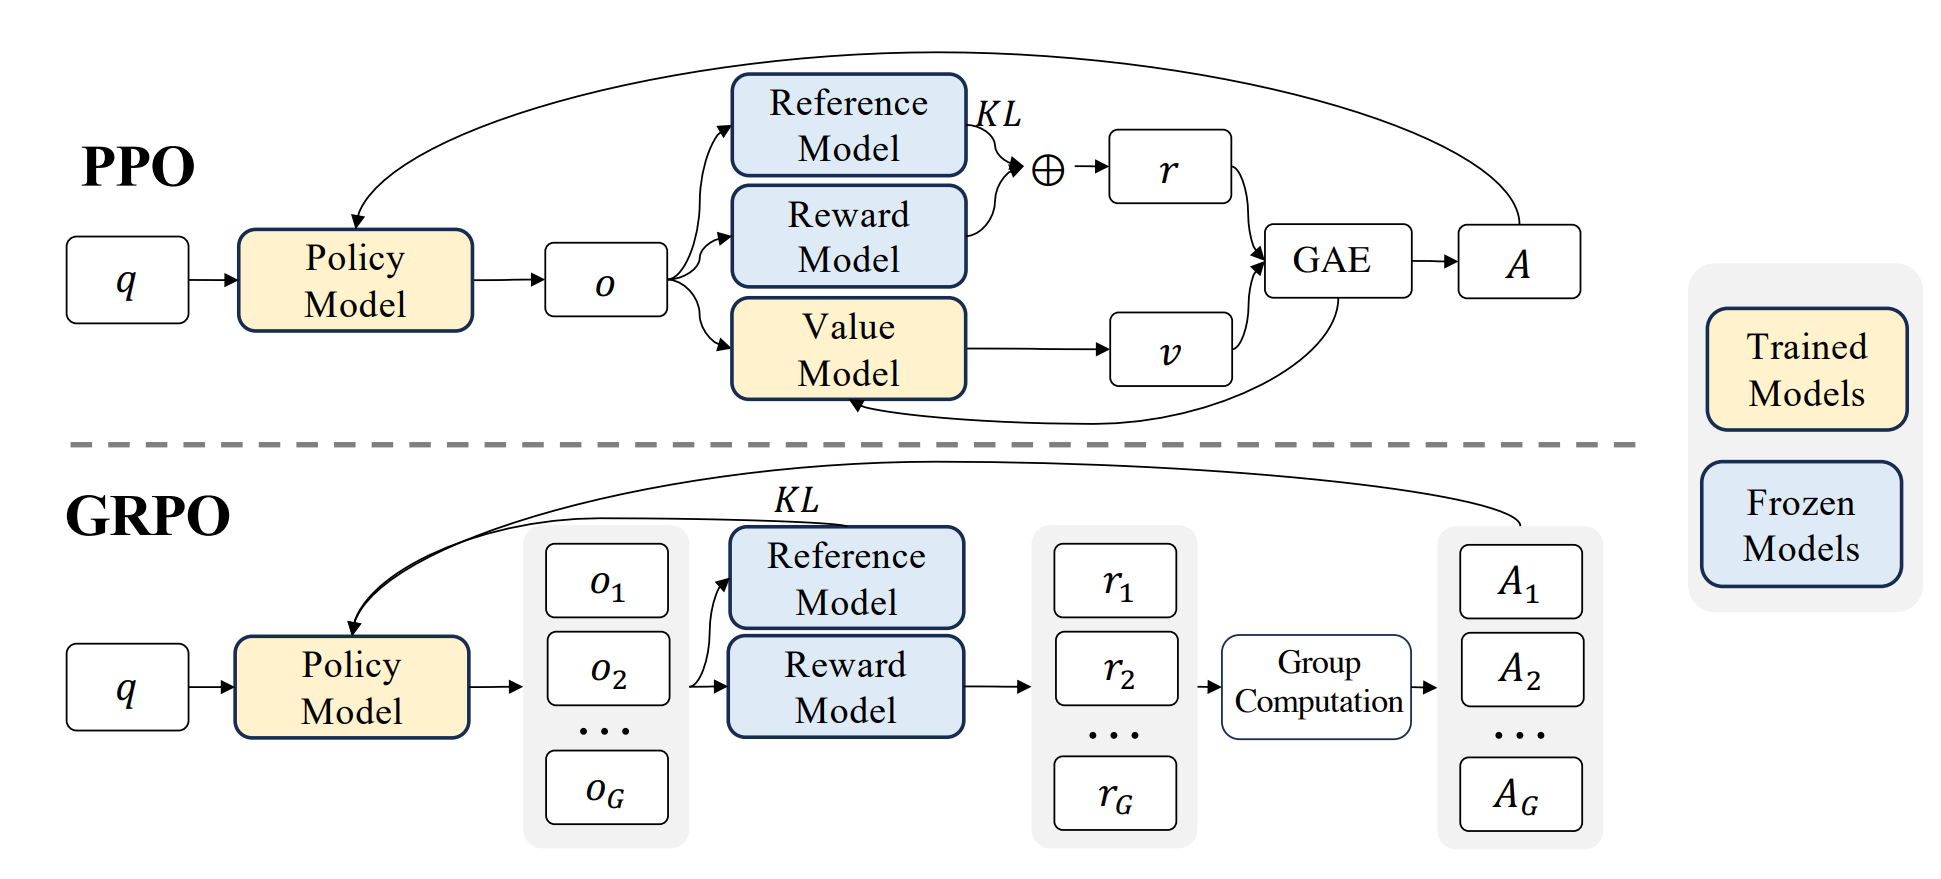
\includegraphics[width=\textwidth]{img/GRPO.png}
            \caption{GRPO算法框架}
        \end{figure}
    \end{columns}
\end{frame}

% 奖励函数设计
\begin{frame}{奖励函数设计}
    \begin{itemize}
        \item \textbf{准确性奖励(权重5)}
        \begin{itemize}
            \item $R_{accuracy} = \exp(-\text{MSE}(y_{pred}, y_{target}))$
            \item 预测数量影响:$R_{final} = R_{accuracy} \times \text{factor}$
            \item 位置误差分析
        \end{itemize}
        \vspace{0.2cm}
        \item \textbf{格式奖励(权重1)}
        \begin{itemize}
            \item 基本结构(0.4分):标签完整性
            \item 分析步骤(0.3分):推理过程
            \item 答案格式(0.3分):输出规范
        \end{itemize}
    \end{itemize}
\end{frame}

% 训练策略
\begin{frame}{训练策略}
    \begin{itemize}
        \item \textbf{模型配置}
        \begin{itemize}
            \item Qwen2.5-1.5B-Instruct模型
            \item 最大序列长度:800 tokens
            \item 温度系数:0.7,top-p:0.9
        \end{itemize}
        \vspace{0.2cm}
        \item \textbf{GRPO参数}
        \begin{itemize}
            \item $\beta$ 系数:0.04
            \item $\epsilon$ 阈值:0.2
            \item 每个输入生成4个候选结果
        \end{itemize}
    \end{itemize}
\end{frame}